\documentclass{natureprintstyle}
%\documentclass{nature}
\bibliographystyle{naturemag}
\usepackage{epsfig,caption}
\usepackage{color}
\usepackage{bm}
\usepackage{graphicx}
\usepackage{longtable}
\usepackage{amssymb}
\usepackage{rotating}
\usepackage{latexsym}
\usepackage{hyperref}
\usepackage{float}

%\usepackage[switch]{lineno}
%\linenumbers

%%%%%%%%%%%%%%%%%%%%%%%%%%%%%%%%%%%%%%%%%%%%%%%%%%%%%%%%%%%%%%%%%%%
% comment for selecting the best figures to go on web for:
%@arxiver{jvds_sami_vsigma_ellip_LOESS_Age_paper.pdf,jvds_sami_vsigma_ellip_LOESS_Age_transform_paper_resubmit.pdf} 
%%%%%%%%%%%%%%%%%%%%%%%%%%%%%%%%%%%%%%%%%%%%%%%%%%%%%%%%%%%%%%%%%%%

%journal commands
\newcommand{\apj}{Astrophys. J.}
\newcommand{\spie}{Proc. SPIE}
\newcommand{\pasp}{Publ. Astron. Soc. Pac.}
\newcommand{\apjs}{Astrophys. J. Supp.}
\newcommand{\araa}{Annu. Rev. Astron. Astrophys.}
\newcommand{\mnras}{Mon. Not. R. Astron. Soc.}
\newcommand{\apjl}{Astrophys. J. Let.}
\newcommand{\aap}{Astron. Astrophys.}
\newcommand{\aj}{Astron. J.}
\newcommand{\nat}{Nature}
\newcommand{\na}{New Astron. Rev.}
\newcommand{\aaps}{A\&AS}
\newcommand{\procspie}{Proc. SPIE}

%%%%%%%%%%%%%%%%%%%%%%%%%%%%%%%%%%%%%%%%%%%%%%%%%%%%%%%%%%%%%%%%%%%
% my commands

\newcommand{\lcdm}{$\Lambda$CDM}
\newcommand{\hst}{{\it HST}}
\newcommand{\efr}{$R_{\mathrm{eff}}$}
\newcommand{\galfit}{{\sc Galfit}}
\newcommand{\mbh}{$\mathcal M_{\rm BH}$}
\newcommand{\lhost}{$L_{\rm host}$}
\newcommand{\mr}{$Mag_{\rm ~R}$}
\newcommand{\jcap}{Journal of Cosmology and Astroparticle Physics}
\newcommand{\halpha}{${\it H}\alpha$}
\newcommand{\hbeta}{${\it H}\beta$}
\newcommand{\sersic}{S\'ersic}
\newcommand{\lenstronomy}{{\sc Lenstronomy}}
\newcommand{\reff}{{$R_{\mathrm{eff}}$}}
%\newcommand{\kms}{km~s$^{\rm -1}$}
\newcommand{\kms}{\ifmmode{\,\rm{km}\, \rm{s}^{-1}}\else{$\,$km$\,$s$^{-1}$}\fi}
\newcommand{\sigstar}{{$\sigma_*$}}
\newcommand{\mstar}{{$M_*$}}
\newcommand{\Mgii}{Mg$_{\rm II}$}
\newcommand{\Civ}{C$_{\rm IV}$}
\newcommand{\farcs}{\mbox{\ensuremath{.\!\!^{\prime\prime}}}}% fractional arcsecond symbol: 0.''0
%%%%%%%%%%%%%%%%%%%%%%%%%%%%%%%%%%%%%%%%%%%%%%%%%%%%%%%%%%%%%%%%%%%

\newcommand{\ding}[1]{\textcolor{red}{[{\bf Xuheng}: #1]}} 

\title{
%From predictions to observation: scaling relations between supermassive black holes and their host galaxies at $1< z<2$
A successful observational test of black hole and galaxy co-evolution models since $z\sim1.7$
%The first comparison between the observation and simulation of the scaling relations between supermassive black holes and their host galaxies at $1.2< z<1.7$
}
\author{Xuheng Ding$^{1,2}$, 
Tommaso Treu$^{1}$, 
John Silverman$^{3, 4}$,
Aklant K. Bhowmick$^{5}$,
N. Menci$^{6}$,
Tiziana Di Matteo$^{5}$,
et. al.
}

\begin{document}

\maketitle

\let\thefootnote\relax\footnote{
\begin{affiliations}
\item {Department of Physics and Astronomy, University of California, Los Angeles, CA, 90095-1547, USA} 
\item {School of Physics and Technology, Wuhan University, Wuhan 430072, China}
\item {Kavli Institute for the Physics and Mathematics of the Universe (WPI), The University of Tokyo, Kashiwa, Chiba 277-8583, Japan}
\item {Department of Astronomy, School of Science, The University of Tokyo, 7-3-1 Hongo, Bunkyo, Tokyo 113-0033, Japan}
\item{McWilliams Center for Cosmology, Dept. of Physics, Carnegie Mellon University, Pittsburgh PA 15213, USA}
\item{INAF Osservatorio Astronomico di Roma, via Frascati 33, I-00078 Monteporzio, Italy}
\end{affiliations}
}

\begin{abstract}
Supermassive black holes (BH) harbor at the center of galaxies with their masses (\mbh) correlated to the properties of the host galaxies, including absolute magnitude ($Mag$) and stellar mass (\mstar) known as scaling relations (i.e., \mbh-\lhost, \mbh-\mstar). 
 %Observational results have indicated evidence that this correlation evolves with cosmic time, suggesting a scenario that the BH growth predates their host. In theory, positive evolution of BH is also predicted by several simulation projects independently.
So far, the simulations have reproduced these relations which have a good agreement to the observational sample from local to intermediate redshift ($z<1$). It is crucial to extend this study to higher redshift ($z>1$), where the predicted relations are more sensitive to the initial assumptions and any inconsistency would help to pinpoint the incorrect ones.
To this end, we use a sample of 32 X-ray-selected broad-line (type-1) AGNs at $1.2 < z < 1.7$ ($\sim 8.5-10$ billion years ago) to make a direct comparison to the predicted sample using two independent state-of-the-art simulation projects: MassiveBlack-II (MBII) and semi-analytic models (SAM). We adopt \hst\ to take the  AGN image in multi-bands to derive the trustworthy host galaxies properties and use the reliable broad \halpha\ emission lines by Subaru/FMOS to estimate the \mbh. Taking the selection bias into account, %by adopting the same selection function to choose the simulating sample,
we find that both MBII and SAM agree well with the data, in terms of the central distribution. However, when taking the measurement uncertainty into account and comparing the scatter, the observations are more consistent with the MBII sample ($\sim0.3$~dex), than the SAM one ($\sim0.7$~dex). In this respect, our observational constraints are able to distinguish the two models, indicating that the recipe by MBII (AGN feedback driven) is more rather than the SAM one (galaxy interaction driven). Moreover, the intrinsic scatter of our high-$z$ sample is not larger than the local sample, which is against the central limit theorem (a purely stochastic process). To some extent, our result attests that there has to be a causal link between SMBH and its host galaxy to induce an ordering so that the more massive black holes are tightly linked to the more massive galaxies.

\end{abstract}

%\section{Introduction}
The discovery of the correlations between the masses (\mbh) of supermassive black holes (SMBH) and the properties of their host galaxies, such as absolute magnitude ($Mag$) and stellar mass (\mstar), indicates that the growth of SMBH could be connected to its host galaxy formation~\cite{Mag++98, F+M00, M+H03, H+R04, Gul++09}. So far, the origin that drives this connection is still unknown, due to the daunting range of scales between the dynamical sphere ($\sim$pc) of the SMBH and their host galaxy ($\sim$10 kpc). A dominant interpretation is so-called AGN feedback, assuming that a small fraction of AGN energy injects to their surrounding gas that regulates the growth of SMBH and its host galaxy. In this scenario, the activity of AGN accretion heats and unbinds significant fractions of the gas and inhibits star formation. In addition, there are other models that have been proposed that the connection between SMBH and their hosts are connected not in a direct manner but assuming that they share a common gas supply~\cite{Cen2015, Menci2016}. Furthermore, without any physical mechanisms, it has been proposed that the statistical convergence from galaxy assembly alone (i.e., dry mergers) may reproduce the observed correlations~\cite{Peng2007, Jahnke2011, Hirschmann2010}. In this central limit theorem, a stochastic cloud at high-$z$ (higher scatter) would end up with the scaling relations (lower scatter) as observed today.

To understand this connection, recent works~\cite{Park15, Tre++07, Bennert11, Woo++08} have analyzed the scaling relations to intermediate redshift {($0.3<z<1$)} by studying the active galactic nuclei (AGN) using {\it Hubble Space Telescope} ({\it HST}) and found an evolution that the growth of SMBHs predated to their host galaxies. However, the observational evidence of evolution at high-$z$ is under debated as it relies on our understanding of systematic uncertainties and selection effects~\cite{Lauer2007}. It has been realized that the improper way to consider the uncertainties and selection effects could result in an {\it apparent} evolution and result in an overestimate of the evolution\cite{Volonteri2011}.

%Why comparison between data and model.
%Summary of recently works.
%The reason to extend to high redshift.
Simulation models are effective to help understand this connection and rule out the theories/assumptions which could not be verified by the observations. In simulation test, the systematic uncertainties and selection bias would be easy to account for. Recent studies by several simulation projects have made predictions which are in good agreement with the observations at the intermediate redshift range ($z<1$). For example, the state-of-the-art cosmological hydrodynamical simulations of structure formation (MassiveBlackII) have compared the predicted scaling relations to the \hst\ observation at $0.3<z<1$ and predict a positive evolution that SMBH growth predates the host galaxy~\cite{DeG++15}. Several others works have investigated the scaling relations using large-volume simulations, resulting in well matches to the local relation with some redshift evolution, including approaches using the Magneticum Pathfinder SPH Simulations~\cite{Steinborn2015}, the Evolution and Assembly of GaLaxies and their Environments (EAGLE) suite of SPH simulations~\cite{Schaye2015}, and Illustris moving mesh simulation\cite{Sijacki2015, Vogelsberger2014}. Besides hydrodynamic simulations, the semi-analytic models~\cite{Menci2014, Menci2016} also made remarkable progress and recovered the local scaling relations~\cite{Kormendy13}. However, to date, the comparisons to the observed scaling relations by high-resolution \hst\ imaging sample are still limited within $z<1$ due to the limitation of the observations.

% The work that we want to do
	%Sample selection
	%The advantage of our measurements
	%Compare to which simulation? (some introduction)
	%Any expectation?
	%mention the scatter.
To extend the range, we studied a sample of 32 \hst-observed AGN systems at redshift range $1.2<z<1.7$ from three X-ray coverage fields, including COSMOS~\cite{Civano2016}, (E)-CDFS-S~\cite{Lehmer2005, Xue2011}, and SXDS~\cite{Ueda2008}. The redshift range of our targets is chosen to be high enough ($z>1$) to detect the existence of the evolution offsets and make the comparison to the models, while low enough ($z<2$) to limit the effect of surface brightness dimming. We selected our AGN sample in a well-defined window as in Figure~\ref{fig:AGN_select}, based on the \mbh\ and Eddington ratio \ding{Do we plot figure1 here again, or cite to the QSO I paper?}. As shown, the \mbh\ are well below the knee of the BH mass distribution to avoid strong selection bias. In addition, the Eddington ratios are mostly above $0.1$ to ensure the homogeneity.

We measure reliable \mbh\ and host properties to overcome the systematic. Specifically, the \mbh\ of our sample are estimated using the published near-infrared spectroscopic observations of the broad \halpha\ emission lines, which removes the systematic with \Mgii\ or \Civ. For the inference of properties of the host galaxies, the X-ray selected sample has lower nuclear-to-host ratios at IR band, which facilitates the inference of the host light. We employ the \hst/WFC3 to obtain high-resolution (0\farcs0642 per pixel) imaging data and adopt the state-of-the-art technique to perform the 2-D flux profile decomposition to infer the light of the host galaxy. Moreover, 21/23 systems have \hst/ACS imaging data, which enable us to assess the colors of the host, hence the rest frame R-band magnitude (\mr) and stellar mass (\mstar) (see Methods). 
%We furthermore combining them with the ground-based photometry to carry out the SED fitting, and thus derive the reliable host rest-frame R band luminosity and stellar mass.

\begin{figure}[t]
\includegraphics[width=0.9\linewidth]{AGN_selection.pdf}
\caption{The selection for the 32 AGN sample. The top and right panels are the BH mass function and Eddington ratio function. \ding{More descriptions are needed if Figure1 is finally decided to show.}
}
\label{fig:AGN_select}
\end{figure}

To make the comparison, we adopt two independent simulation projects, including MassiveBlack-II (MBII)~\cite{Khandai2015} and semi-analytic models (SAM)~\cite{Menci2014}. These two models are based on independent model strategies, i.e., hydrodynamic simulation for MBII and semi-analytic model for SAM, respectively. The MassiveBlack-II (MBII) simulation is the highest resolution at the size of a comoving volume $V_{\rm box} = (100~{\rm Mpc}~h^{-1})$, including a self-consistent model for star formation, black hole accretion, and associated feedback. The large simulation volume enables the simulating objects to evolve independently; the high enough mass and spatial resolution meet the requirements for the object details. On the theoretical side, aimed, high-resolution N-body simulations can study specific galaxy systems. However, understanding the mechanism of the scaling relation requires an analytical description of such processes to be implemented into existing semi-analytic models, such as SAM. In previous works~\cite{Huang2018, DeG++15, Khandai2015, Bhowmick2019, Menci2014, Menci2016}, MBII and SAM have made high successful predictions, and we refer the interested readers to these works for more details.

%\section*{Results}
%Selection effect into account
Based on MBII project, we collect a sample of simulated AGNs at $z=1.5$ and compare their predicted scaling relations to the observed ones. We take the measurement uncertainty and the selection effect into account to ensure a fair comparison,  with the following process. First, we inject the random noise to the simulated sample to mimic the scattering effect caused by the uncertainty. The assumed uncertainties are set to be comparable to the realistic levels, i.e., $\Delta$\mbh =0.4~dex, $\Delta$\mr=0.3~dex, $\Delta$\mstar=0.17~dex, and $\Delta L_{\rm bol}$=0.03~dex, respectively. We then select the sample that falls into the same targeting window to mimic the sample selection process, as shown in Figure~\ref{fig:selectfunc}. We investigated the predicted scaling relations, including \mbh-\mr\ and \mbh-\mstar, and compared them to the observational constraints, as shown in Figure~\ref{fig:MBII_comp}. From a quick glimpse, one can see that the samples are overlapped with each other, showing a sign of agreement. To quantify the level of agreement, we perform the linear regression to fit the simulated relations and estimate the best-fit inference and 1$-\sigma$ confidence interval. We use the same slope value to obtain the best-fit intercept value for the observed sample. We find that for the \mbh-\mr\ relation, the linear fitting results are almost identical, with only $0.06$~dex mismatch. For the \mbh-\mstar\ relations, the mismatch ($0.15$~dex) is small and far below 1$-\sigma$ level. Furthermore, we compare the scatter of the sample by calculating the standard derivation of the residual in the linear regression. We find that the simulations and the observations have the same scatter level $0.3$~dex. Considering that the simulated samples have the same uncertainty and the selection effect, we expect the intrinsic scatter of the scaling relations are similar, which is $0.25$~dex (see METHODS).

\begin{figure}[t]
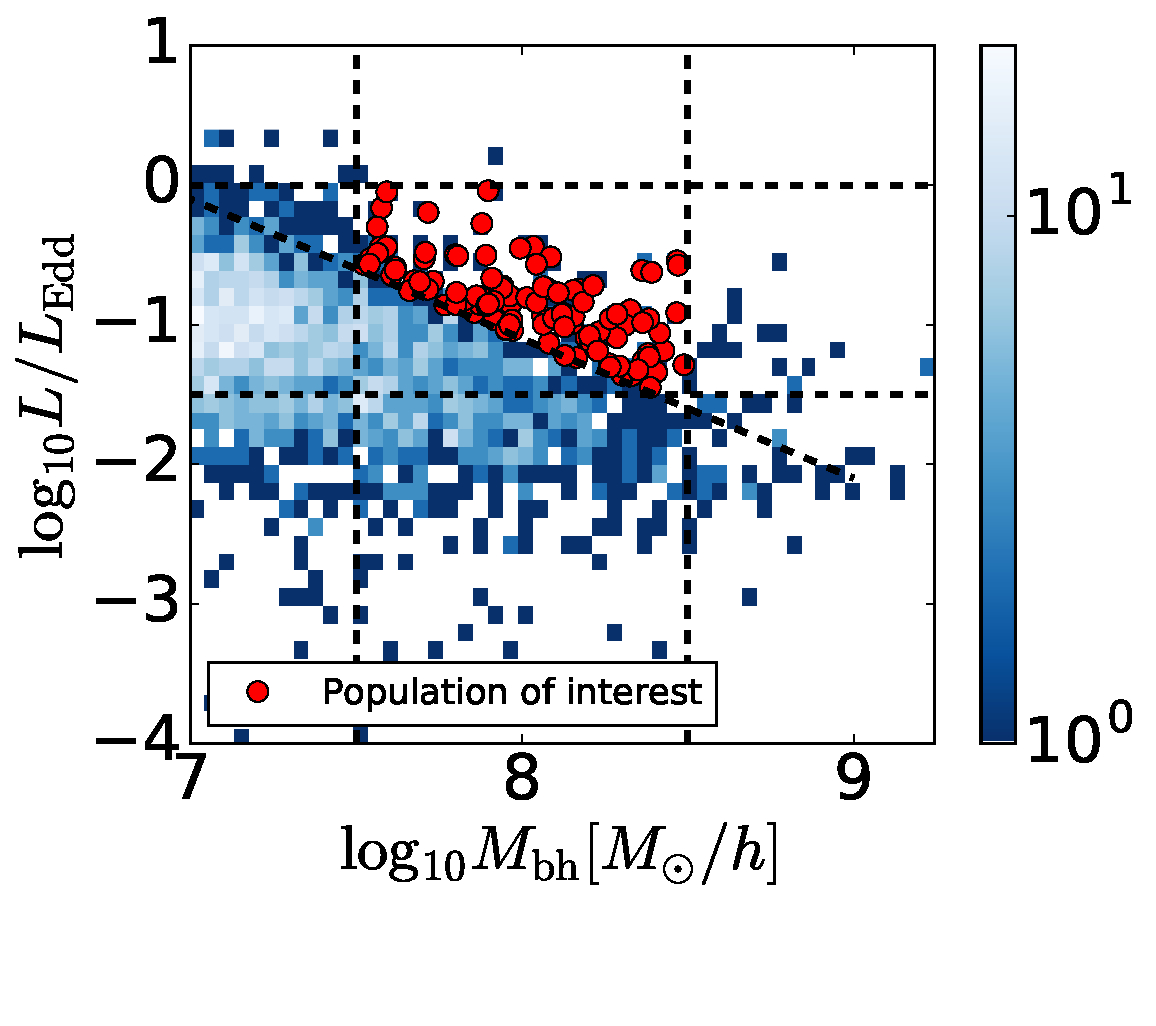
\includegraphics[width=1.0\linewidth]{MBII_selectfunc.pdf}
\caption{The same selection window as adopted for selecting the MBII simulated sample. The yellow background clouds shows the overall sample at $z=1.5$. We add the random uncertainty to the simulation and select the ones fall into the targeting region (i.e. red colored). The yellow dots are the HST sample.}
\label{fig:selectfunc}
\end{figure}
%comparison to simulation (flux ratio also)

\begin{figure*}[t]%[!b]
\begin{tabular}{c c}
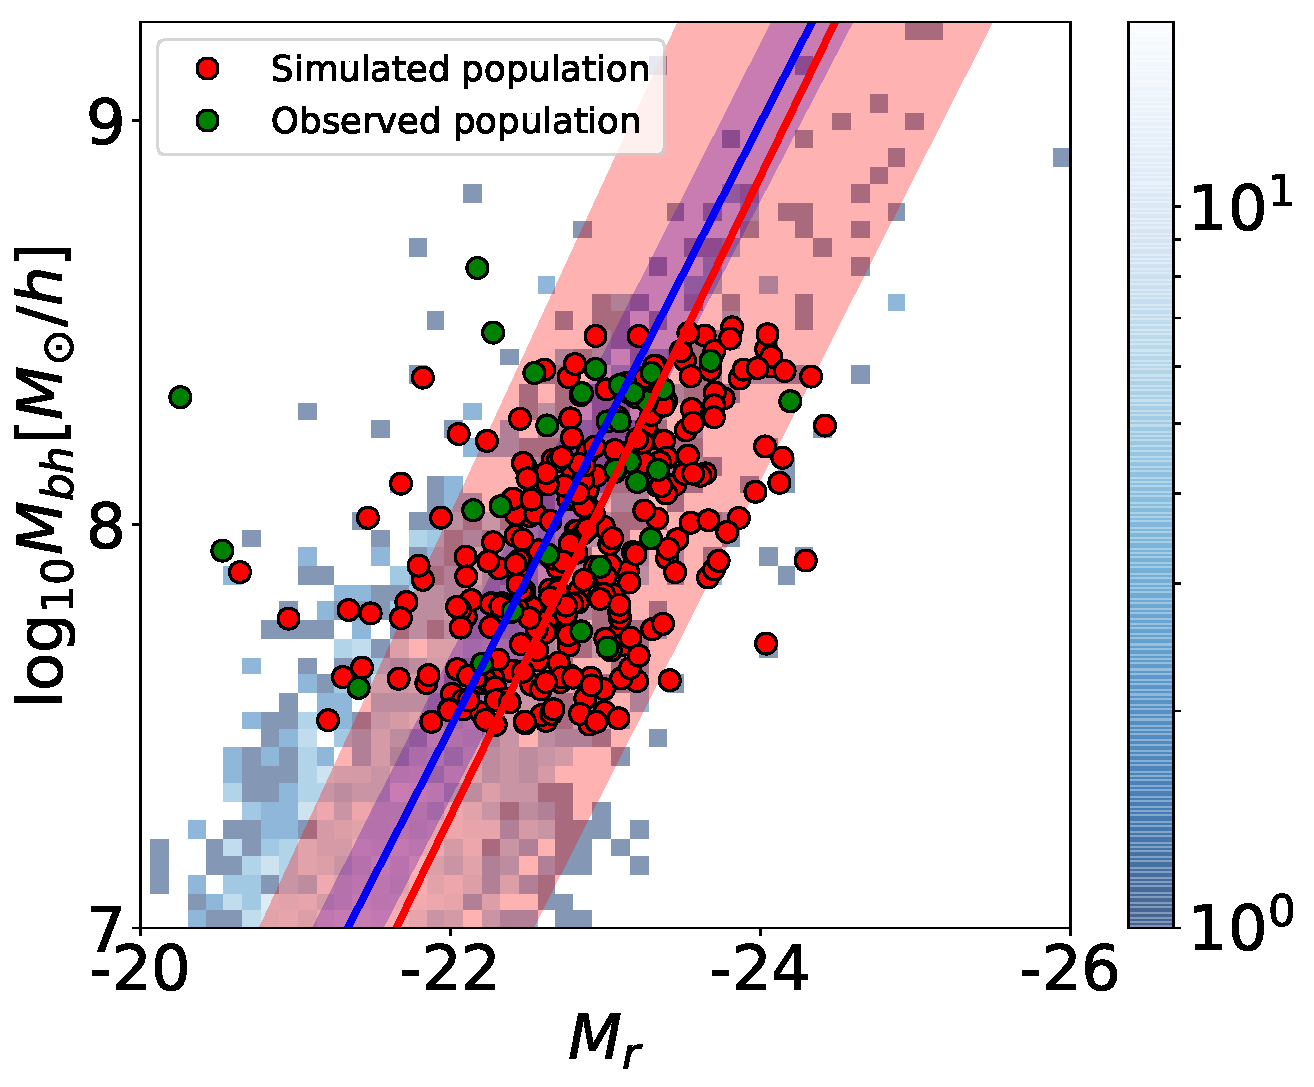
\includegraphics[width=0.5\linewidth]{MBII_ML.pdf} &
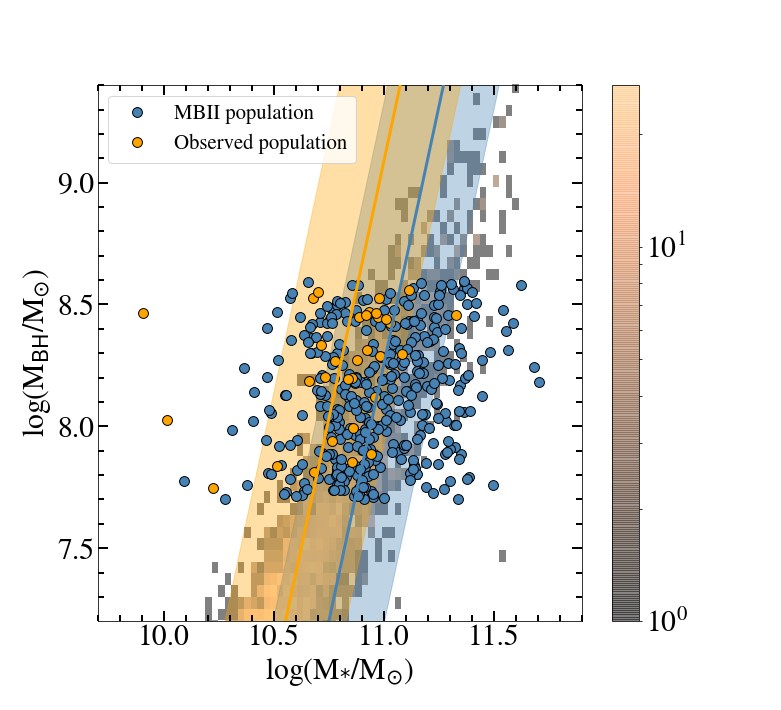
\includegraphics[width=0.5\linewidth]{MBII_MM.pdf} \\
\end{tabular}
\caption{  In the left and right panel, we present the \mbh-\mr\ and \mbh-\mstar\ correlation between the observed scaling relations (yellow dots) and the predicted samples (red dots) by the MBII simulation, respectively. The MBII predicted sample is treated to have the same uncertainty and selection effect as the observational ones. The red line is the best-fit result for the simulated sample, with the red-color region indicating the $1-\sigma$ confidence interval. We use the same slope value to fit for the observed sample, and the green line shows the best-fit result. The yellow grids in the background are the overall sample that predicted in the MBII simulation.  %{\bf For the right panel, I currently adopt a 3 Gyrs template for the HST sample...}
}
\label{fig:MBII_comp}
\end{figure*}

We also make comparisons of our observed scaling relations to the predictions by the SAM model. Rather than N-body simulation, which produces individual simulating objects, the SAM model uses the density clouds to describe the possibility of the samples. We consider the sample at $z=1.5$ epoch for two sample sets, including the overall sample and the selected sample, as shown in Figure~\ref{fig:SAM_comp}. We find that considering the selecting effect, the direct prediction by SAM is well matched to the observed relations.
%We do not estimate the scatter for SAM model, but visually see that the observed relations are mostly located on top of the hot cloud, showing that the observed scatter should not be larger than the model one. \ding{This is not right yet. But if consider the scatter in the same way, the SAM have large scatter?}
Yet this is not a proper comparison since the direct sample from SAM does not include the scattering effect by the measurement uncertainty. To make a valid comparison, we first randomly generate the overall sample for SAM based on the possibility clouds. Then, same as MBII's case, we inject the random uncertainty to the sample to take the uncertainty effect into account and select the sample the selection window. The resulting comparisons are shown in Figure~\ref{fig:SAM_comp_withnoise}. We find that the best-fit result by the SAM model is well matched to the observation. However, the scatter of the SAM model are overwhelmingly larger ($0.7$~dex) than the observation. This larger scatter is a combination result by the SAM distribution, uncertainty, and selection effect.  


\begin{figure*}[t]%[!b]
\begin{tabular}{c c}
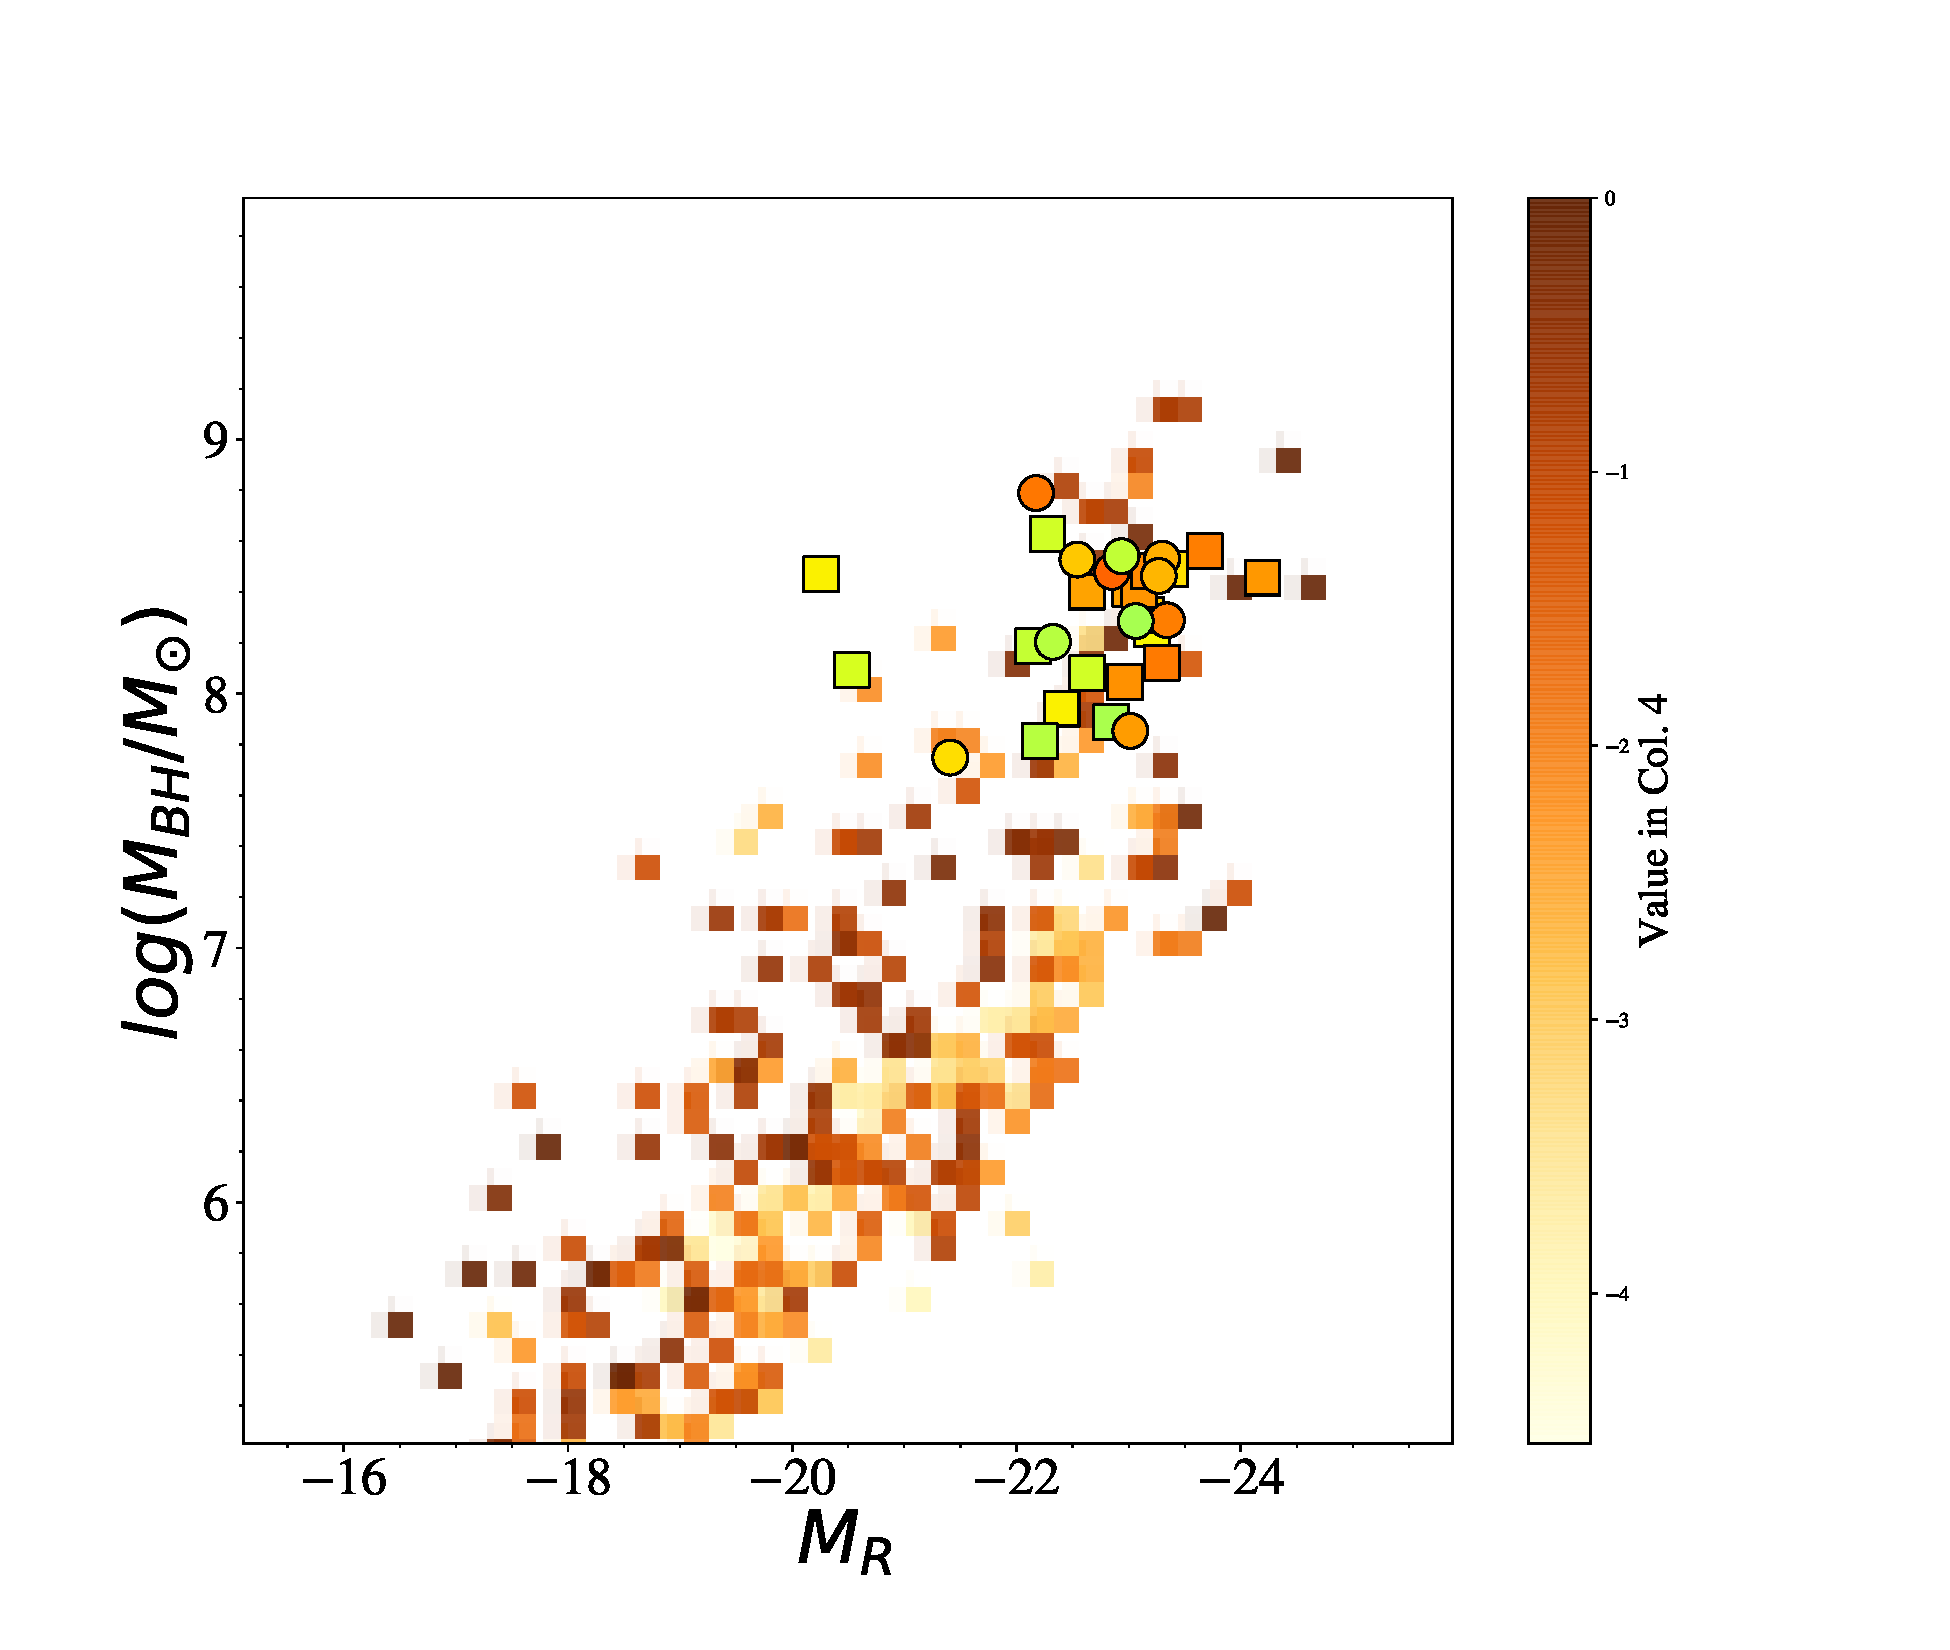
\includegraphics[trim = 0mm 0mm 24mm 0mm, clip, width=0.45\linewidth]{SAM_ML.pdf} &
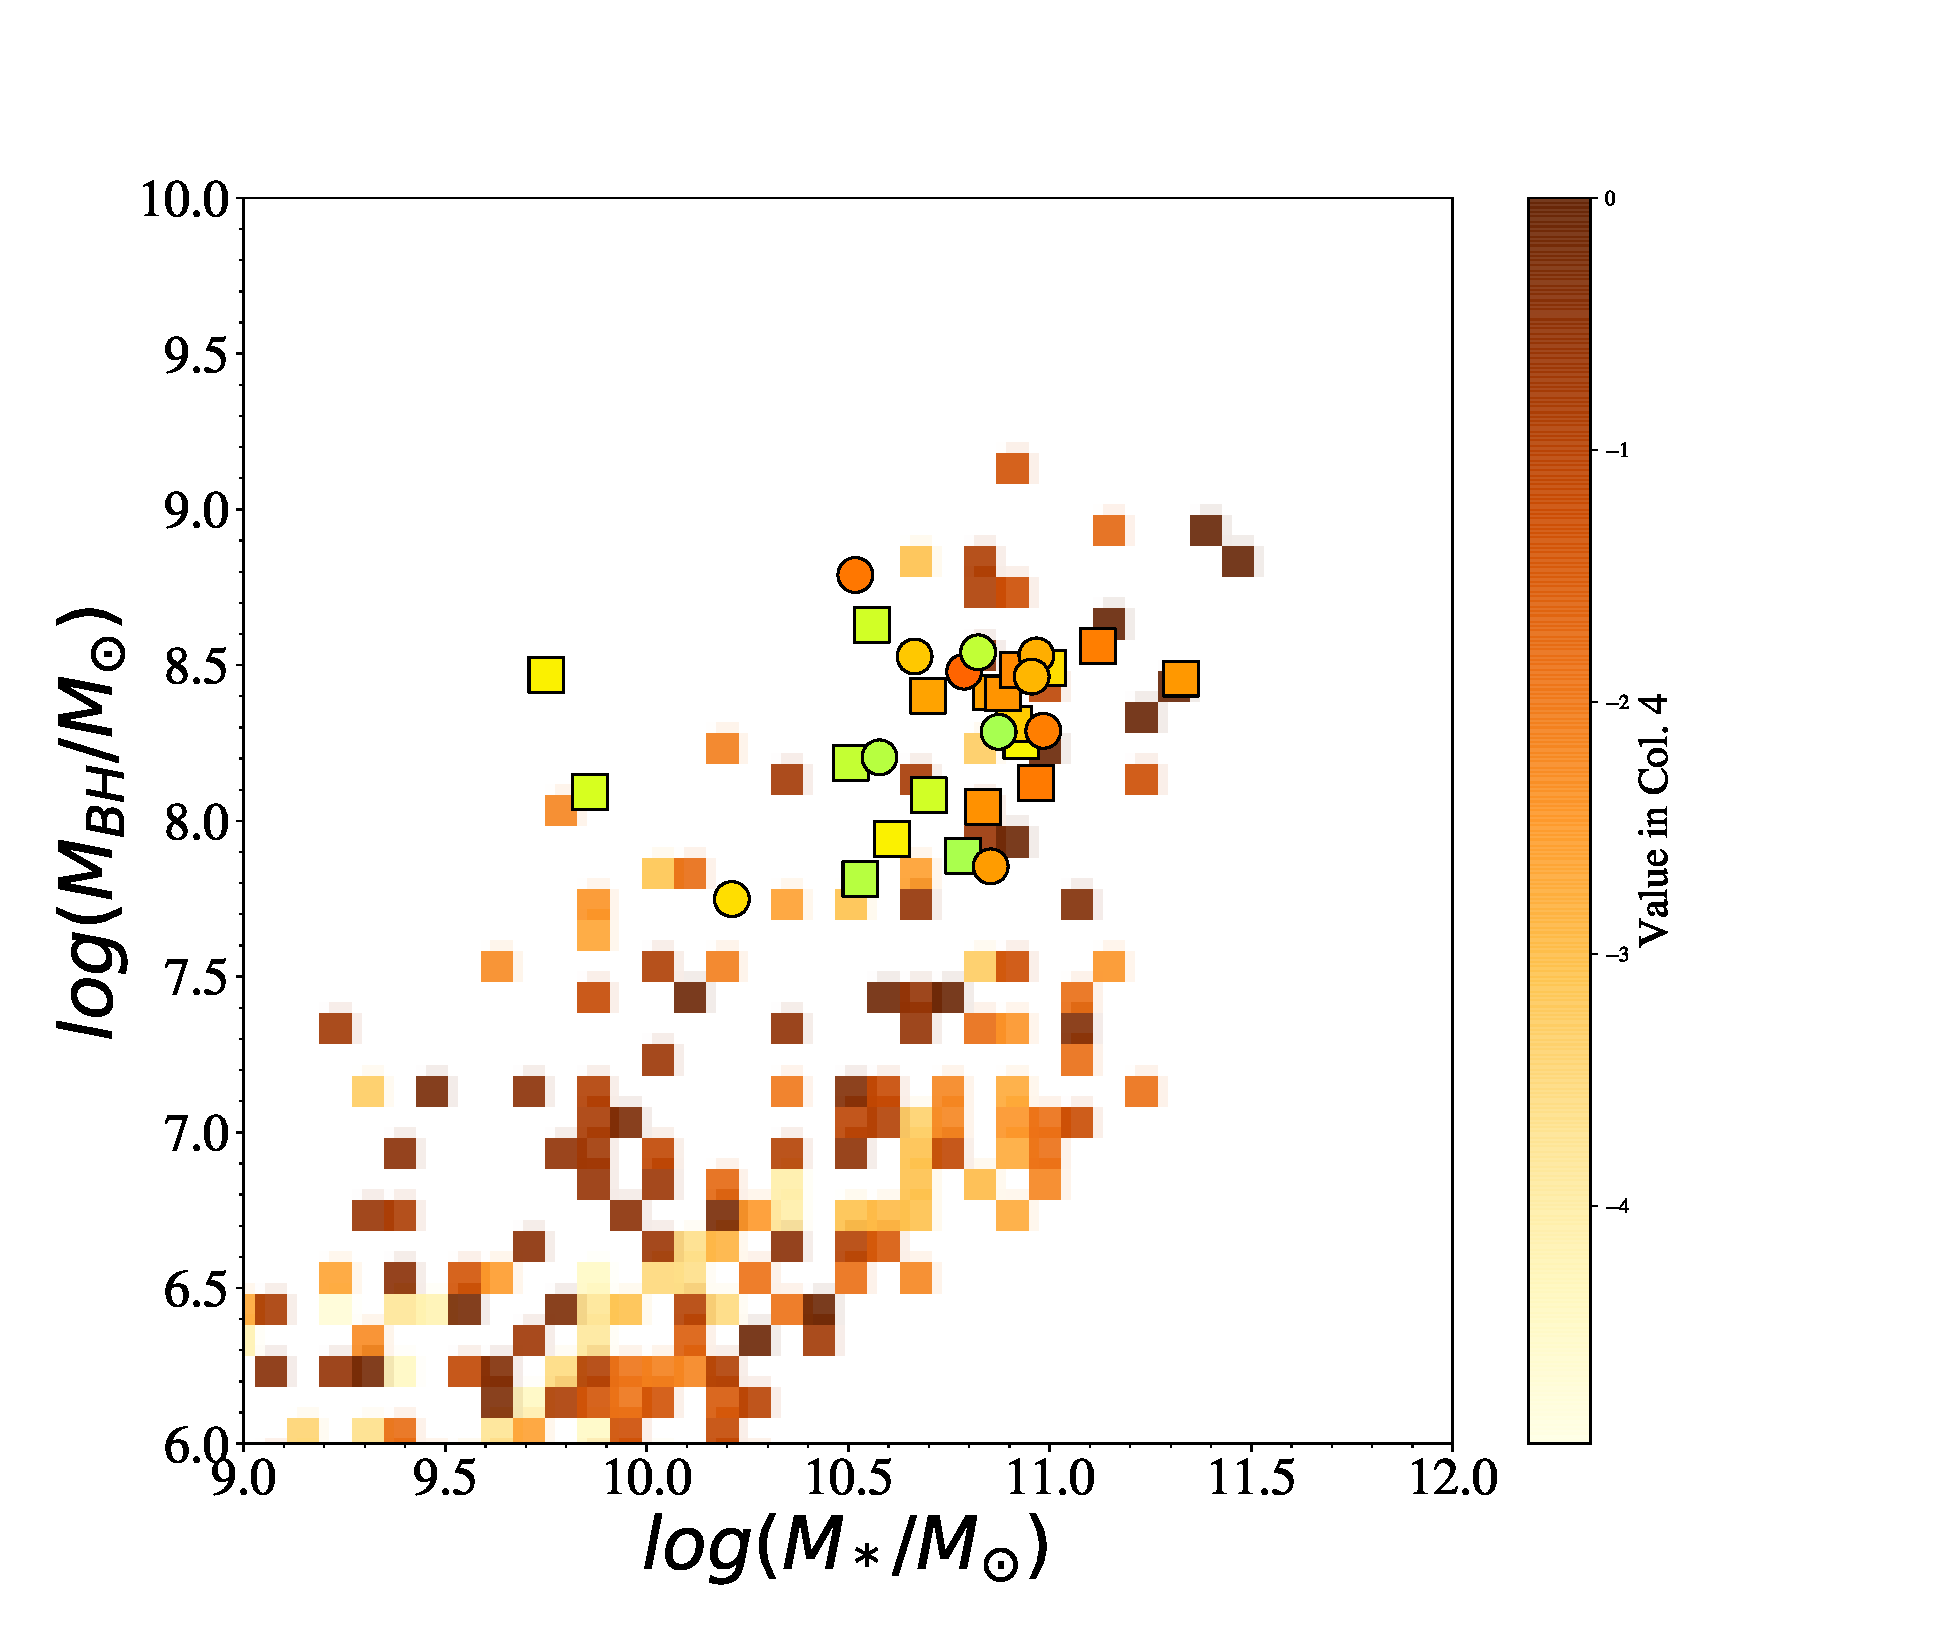
\includegraphics[trim = 30.5mm 0mm 0mm 0mm, clip, width=0.45\linewidth]{SAM_MMstar.pdf} \\
\end{tabular}
\caption{Similar to the Figure~\ref{fig:MBII_comp}, but for a direct comparison to the observation using SAM's model. The blue background contours show the possibility distribution for the overall sample, and the red contours indicate the distributions after considering the selecting effect. We presented our observational data as yellow dots. Note that this comparison has not taken the measurement uncertainties into account yet. 
}
\label{fig:SAM_comp}
\end{figure*}

\begin{figure*}[t]%[!b]
\begin{tabular}{c c}
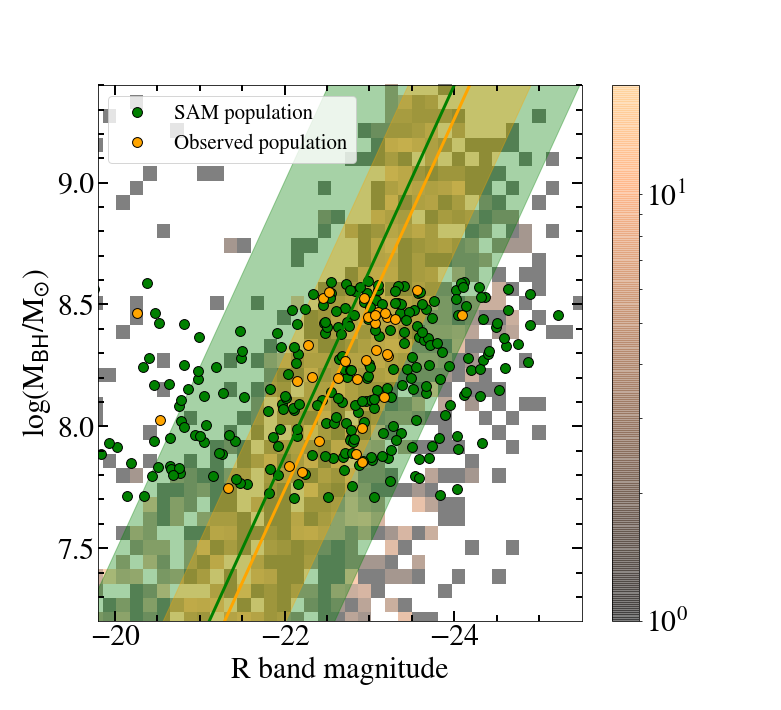
\includegraphics[width=0.45\linewidth]{SAM_ML_consider_nois.pdf} &
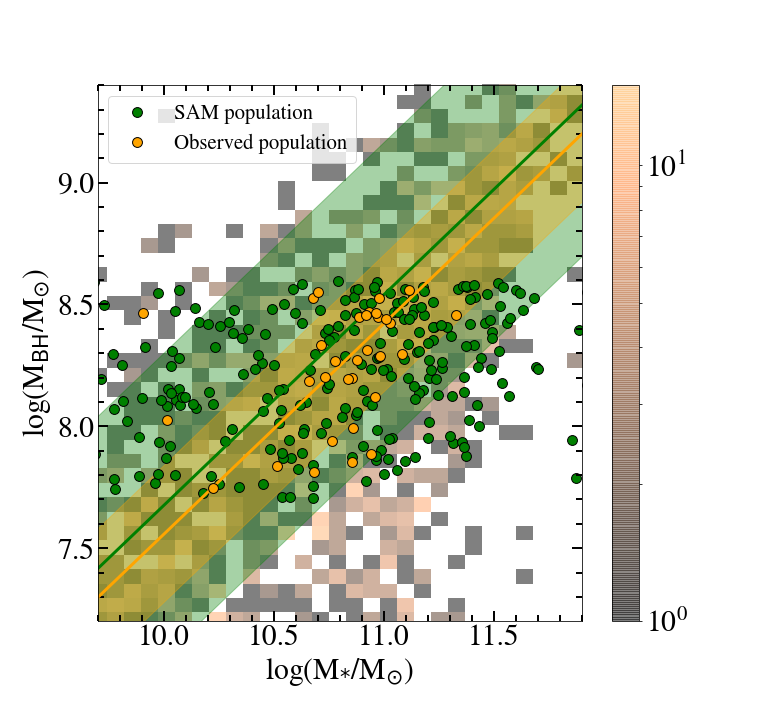
\includegraphics[width=0.45\linewidth]{SAM_MM_consider_nois.pdf} \\
\end{tabular}
\caption{Same as the Figure~\ref{fig:MBII_comp}, but for the SAM models.}
\label{fig:SAM_comp_withnoise}
\end{figure*}

 \ding{We can put this paragraph into Method or even delete.} To test if any unexpected selection effects exist, we compare the distribution of the host-total flux ratio among these three samples. For the observed sample, we calculate the flux ratio at the imaging band, i.e., \hst/WFC3. For the simulated sample, we consider the AGN bolometric correction~\cite{Elvis1994} to estimate the AGN light flux at WFC3/F125W band. We compare their host-total flux histogram distribution in Figure~\ref{fig:comp_hist} and see that the three samples are well matched each other. The median values for the flux ratio distribution of the observed, MBII, SAM sample are $37.3\%$, $32.3\%$, and $42.8\%$, respectively. We perform the Kolmogorov-Smirnov (KS) test the inferred p-values are 0.34 (for observed -- MBII) and 0.14 (for observed -- SAM), respectively. This result indicates the three samples have similar host-to-total light distribution.

\begin{figure}[t]
\includegraphics[width=0.9\linewidth]{comp_host_ratio.pdf}
\caption{The comparison histogram of the host ratios among three referred samples, median value indicated. The same selection effect are considered for the simulation sample.
}
\label{fig:comp_hist}
\end{figure}

In terms of their central distribution, the MBII simulation and SAM model both demonstrate an excellent agreement to the observational constraints. However, when considering the scattering effect by the measurement uncertainty, the scatter in MBII simulation is consistent to the observational one ($\sim0.3$~dex) and SAM sample has much larger scatter ($\sim0.7$~dex). Given that the two models adopt very different assumptions, recipes, and initial conditions, our result shows that the mechanism (AGN feedback driven) by MBII is more favorable. An explanation for the larger scatter in the SAM model is that its BH feeding is by merger driven with more stochasticities in the scaling relations. In particular, the SAM cloud extends to the high \mbh\ with low stellar mass, which may not exist. \ding{To Nicola: is that possible to change the assumption in SAM to make the relations tighter?} The consistency between MBII and observations indicates that there has to be a causal link between SMBH and its host galaxy to generate an ordering during their evolution; as a result, more massive BHs are linked to more massive galaxies {\it tightly}.

Without any physical mechanisms, the central limit theorem~\cite{Peng2007, Jahnke2011, Hirschmann2010} assumes that the scaling relations are caused by the random merger from a stochastic cloud at earlier universe. In this scenario, the scatter of the scaling relations has to be larger with the increasing of redshift. However, the observed scatter of our high-$z$ sample do not present this feature. In fact, our inferred intrinsic scatter of the observed sample is $\sim0.25$~dex, which is no more than the typical scatter at local relations in the literature ($\sim0.35$~dex)~\cite{Kormendy13, Gul++09}. Of course, the intrinsic scatter of our high-$z$ sample could be inaccurate, since we use the MBII overall sample as a proxy to estimate our value.
Also, the observed \mbh\ are estimated using the robust \halpha\ line, which could have lower uncertainties level than expected (i.e., $\Delta$\mbh$<0.4$~dex), resulting in an overestimating of the error-budget and thus underestimating of intrinsic scatter. Still, the evidence of the low scatter in our measurements is likely to be true, which is against the central limit theorem and suggests that the physical mechanisms between the SMBH and its host galaxy are likely to exist. 

Extending the redshift range of this study would be very beneficial to this study, giving that the scaling relation in the simulations shows different evolution at the different stage of the universe. For higher redshift, the {\it James Webb Space Telescope} may provide high-quality imaging data of AGNs at redshift up to $z\sim7$. In the low redshift Universe, wide-area surveys with Subaru/HSC, LSST, and WFIRST offer much promise to build samples for studying these mass ratios and dependencies on other factors (e.g., environment).

%\textcolor{blue}{The details of the results could be presented.\\
%0. Compare the color of the sample?\\
%1. 2D KS test? \\
%2. More insightful inference from the comparing?
%}

%Discuss the result, What does this mean?

% \textcolor{blue}{If the final results show such feature:}
%The result also shows that the \mbh-\mstar\ relation has less scatter than the \mbh-\lhost\ relation, suggesting that the BH relation with \mstar\ are more fundamental than \lhost.
%This successful experience leads one conjecture that the other prediction by the simulations could likely to be right. For example, regarding the stellar components of galaxy which is the origin that related to the growth of BH, it is likely that the bulge masses are tightly related.

%\section*{Discussion}
%Some discussions should be placed in this section.
%On the observation side:\\
%0. The inferred host flux ratio by SED decomposition is consistent to the 2-D image decomposition, indicating the fidelity of these approaches?\\
%1. HST seems to reach its higher limit. In the future, the JWST is very promising to realize the evolution scenario at even higher redshift.\\
%On the simulation side:
%\\0. Introduce some the other 
%\\1. How do we discuss the role of AGN feedback?.

\begin{center}
{\bf \Large \uppercase{Methods} }
\end{center}

%\textbf{Observation data.} Our 32 new AGN systems are selected from four X-ray coverage fields including COSMOS (Civano et al. 2016), (E)- CDFS-S (Lehmer et al. 2005; Xue et al. 2011), and SXDS (Ueda et al. 2008) at redshift range $1.2<z<1.7$. The X-ray selected sample have low nuclear-to-host ratios, which facilitates the extraction of the host properties. We adopt the \hst/WFC3 infrared channel to derive the high spatial resolution imaging data, to carry out the decomposition of the AGN-host using two-dimensional flux distribution. The details of the \hst\ observation and the study are presented in the companion paper. Moreover, 21/32 systems have \hst/ACS band, together with some other ground-based observations, which would provide the host information in the other bands. In the next section, we infer the reliable K-correction for the rest-frame R band luminosity and the SED to infer the stellar mass. The \mbh\ of our sample have been estimated by \halpha\ and \hbeta\ in the FMOS survey. Comparing to the \Mgii\ and \Civ, the \mbh\ by broad Balmer lines are more trustworthy. The estimated value of the \mbh\ are listed in the companion paper.
%\textcolor{blue}{Do we need to list the \mbh\ and host properties in a table in this paper?}

\textbf{Imaging data, decomposition and inference of host properties.} 
%1. Imaging data. 2. Inferring host light. 3. Color inference. Rest frame R band and stellar mass.
The detailed description for the analysis is in the companion paper (referring as D19). Here we only present a quick overview of this study. We adopted the \hst/WFC3 infrared channel and selected to use the filters F125W $(1.2<z<1.44)$ and F140W $(1.44<z<1.7)$ (according to the redshift of the targets) to observe the imaging data for the 32 AGN systems through the \hst\ program GO-15115 (PI: John Silverman). We obtain six dither exposures with total exposure time $\sim2394s$ and using  {\sc astrodrizzle} software package to co-add the final image with pixel scale as 0\farcs0642. To mitigate the contamination by the background light from both the sky and the detector, we adopt the {\sc photuils} tools to estimate and remove them accurately.

To address the bias which might be raised by the unknown PSF, we manually collect the isolated-unsaturated PSF-stars from the 32 observed fields, to assemble a PSF library for the fitting. To decompose each AGN image, we assume the unresolved active nuclei as the scaled point source and the host galaxy as the \sersic\ profile. We adopt imaging modeling tool \lenstronomy\cite{lenstronomy} to simultaneously fit their 2-D flux distribution, taking each PSF one by one from the library. Based on the reduced $\chi^2$, we are capable of evaluating the performance of each PSF. We adopt the result from the top-ranked-eight PSFs and using the weighting process to obtain the host property, including flux, \reff, \sersic\ index, using a weighted arithmetic mean.

21/32 images in the COSMOS survey also have imaging data in the ACS/F814W with drizzled pixel scale as 0\farcs03, providing us the multi-band information. We decompose the AGN image in the ACS band to obtain the host flux and compare to the WFC3's result to infer the host color. We find that the 1~Gyr template could well match their color, see Figure~5 in D19, from which we estimate the rest-frame R band luminosity and stellar mass. A Salpeter initial mass function is employed consistently to the observed and simulated sample.

%\textbf{SED fitting and host properties}
%We perform the SED fitting to derive the robust physical properties of the host galaxy, including the rest-frame R band luminosity and stellar mass. 
%21/32 AGN systems have rest-frame UV imaging data by \hst-ACS/F814W\cite{Scoville2007}. We perform the same approach to decompose the photometry of the host light at UV. Since the host inference by IR band is superior to the one by UV band, while fitting UV image, we fix the \reff\ and \sersic\ index as the value inferred by \hst/WFC3 to derive the host flux.
%We furthermore combine the \hst\ inference to the ground-based AGN photometry to carry out the SED fitting. \textcolor{blue}{Details and the figures need to be presented.}
%Adopting the best fit SED stellar template to the \hst/WFC3 flux, we derive the \lhost${,_R}$ and \mstar.

%\textbf{Simulations.} 
%Describe the approaches used in the simulation.

\textbf{Linear fitting and scatter comparison}.  
%How the fitting is done. The comparing of the histogram and the KS test. The scatter. Figures.
To quantify the agreement between the simulation and the observation, we use a linear regression to fit their relations and compare the result. Our selection window has a hard cut on the \mbh\ value (i.e., vertical direction in Figure~\ref{fig:MBII_comp}), and thus the scatter on the host galaxies' properties are larger (horizontal direction). Thus, we fit the host's properties (i.e., \mr\ and \mstar) as a function of \mbh. We adopt the {\sc Scipy} package to estimate the best-fit inference and $1-\sigma$ confidence interval for the simulated sample. We then use the sample slope value to fit for the observations. The comparing results are showing in Figure~\ref{fig:MBII_comp} and~\ref{fig:SAM_comp_withnoise}. To estimate the scatter of the sample, we plot the histogram of the residual, i.e., the sample deviation to their best-fit. The result is presented in Figure~\ref{fig:offset_comp}. We find the standard derivation for observed and MBII sample are consistent and both equal to $\sim0.3$~dex; however for SAM the scatter value is much larger ($\sim0.7$~dex).  We perform the KS test between observed and MBII sample and infer the p-value as $\sim0.3$ for both \mbh-\mr\ and \mbh-\mstar\ relations. Considering that the simulation sample has been processed to have the same uncertainty level and selection effect, we expect the MBII sample and the observational sample have the same intrinsic scatter level. We adopt the python package {\sc Linmix} and estimate this intrinsic scatter based on the MBII overall sample, and obtain $0.25$~dex. 

\begin{figure*}[t]%[!b]
\begin{tabular}{c c}
\includegraphics[width=0.45\linewidth]{comp_scatter_ML.pdf} &
\includegraphics[width=0.45\linewidth]{comp_scatter_MM.pdf} \\
\end{tabular}
\caption{The histogram comparison of the scatter using residual value when fit as linear. The standard derivations for these distribution are $\sim0.3$~dex, $\sim0.3$~dex and $\sim0.7$~dex for observed sample, MBII sample and SAM sample, respectively. Compared to the observation and MBII, the scatters are much larger in SAM's prediction. 
}
\label{fig:offset_comp}
\end{figure*}

%%%%%%%%%%%%%%%%%%%%%%%%%%%%%%%%%%%%%%%%%%%%%%%%%%%%%

\section*{References}
\bibliography{references} 


\begin{addendum}
 \item[Acknowledgements] 
Based in part on observations made with the NASA/ESA Hubble Space Telescope, obtained at the Space Telescope Science Institute, which is operated by the Association of Universities for Research in Astronomy, Inc., under NASA contract NAS 5-26555. These observations are associated with programs \#15115. Support for this work was provided by NASA through grant number HST-GO-15115 from the Space Telescope Science Institute, which is operated by AURA, Inc., under NASA contract NAS 5-26555. The authors fully appreciate input from Simon Birrer, Matthew A. Malkan. XD, SB and TT acknowledge support by the Packard Foundation through a Packard Research fellowship to TT. JS is supported by JSPS KAKENHI Grant Number JP18H01251 and the World Premier International Research Center Initiative (WPI), MEXT, Japan. A.S. is supported by the EACOA fellowship.

%
\item[Author Contributions] X.D. carried out the HST data analysis, led the comparison to the simulating models and was the principal author of the paper. T.T. and J.S. designed the HST project and selected the AGN sample. A.B. and T.D. ran the MBII simulation and provide the simulation data. N.M. ran the SAM model and provide and the SAM data. X.D, T.T, J.S., A.B., T.D., and N.M. interpreted the result.

\end{addendum}

%%%%%%%%%%%%%%%%%%%%%%%%%%%%%%%%%%%%%%%%%%%%%%%%%%%%%%%%%%%%%%%%%%%%%%%%%%%%%%%
\section*{Additional information}
%\textbf{Code availability.} The \lenstronomy, which is used to decompose the AGN image  
%The data reduction package used to process the SAM data is available at http://ascl.net/1407.006, and makes use of 2dfdr: http://www.aao.gov.au/science/software/2dfdr. To derive the stellar kinematic parameters and the lick absorption line strengths, we use the publicly available penalised pixel-fitting (pPXF) code from M. Capppellari: {http://www-astro.physics.ox.ac.uk/~mxc/software/\#ppxf}. For the adaptive LOESS smoothing, we use the code from M. Cappellari obtained from: http://www-astro.physics.ox.ac.uk/~mxc/software/\#loess

\textbf{Data availability.} All the inference of the AGN properties are presented in the companion paper.
%All reduced data-cubes in the GAMA fields used in this Letter are available on: http://datacentral.aao.gov.au/asvo/surveys/sami/, as part of the first SAMI Galaxy Survey data release. Stellar kinematic data products will become available in the second SAMI Galaxy Survey data release. 

\textbf{Correspondence and requests for materials} should be addressed to X.D.~(email:dxh@astro.ucla.edu).

%%%%%%%%%%%%%%%%%%%%%%%%%%%%%%%%%%%%%%%%%%%%%%%%%%%%%%%%%%%%%%%%%%%%%%%%%%%%%%%


%\clearpage
%\newpage
%\onecolumn
%\begin{center}
%{\bf \Large \uppercase{Supplementary information} }
%\end{center}
%
%\setcounter{figure}{0}
%\vspace{2cm}
%
%\begin{figure}[!h]
%\begin{center}
%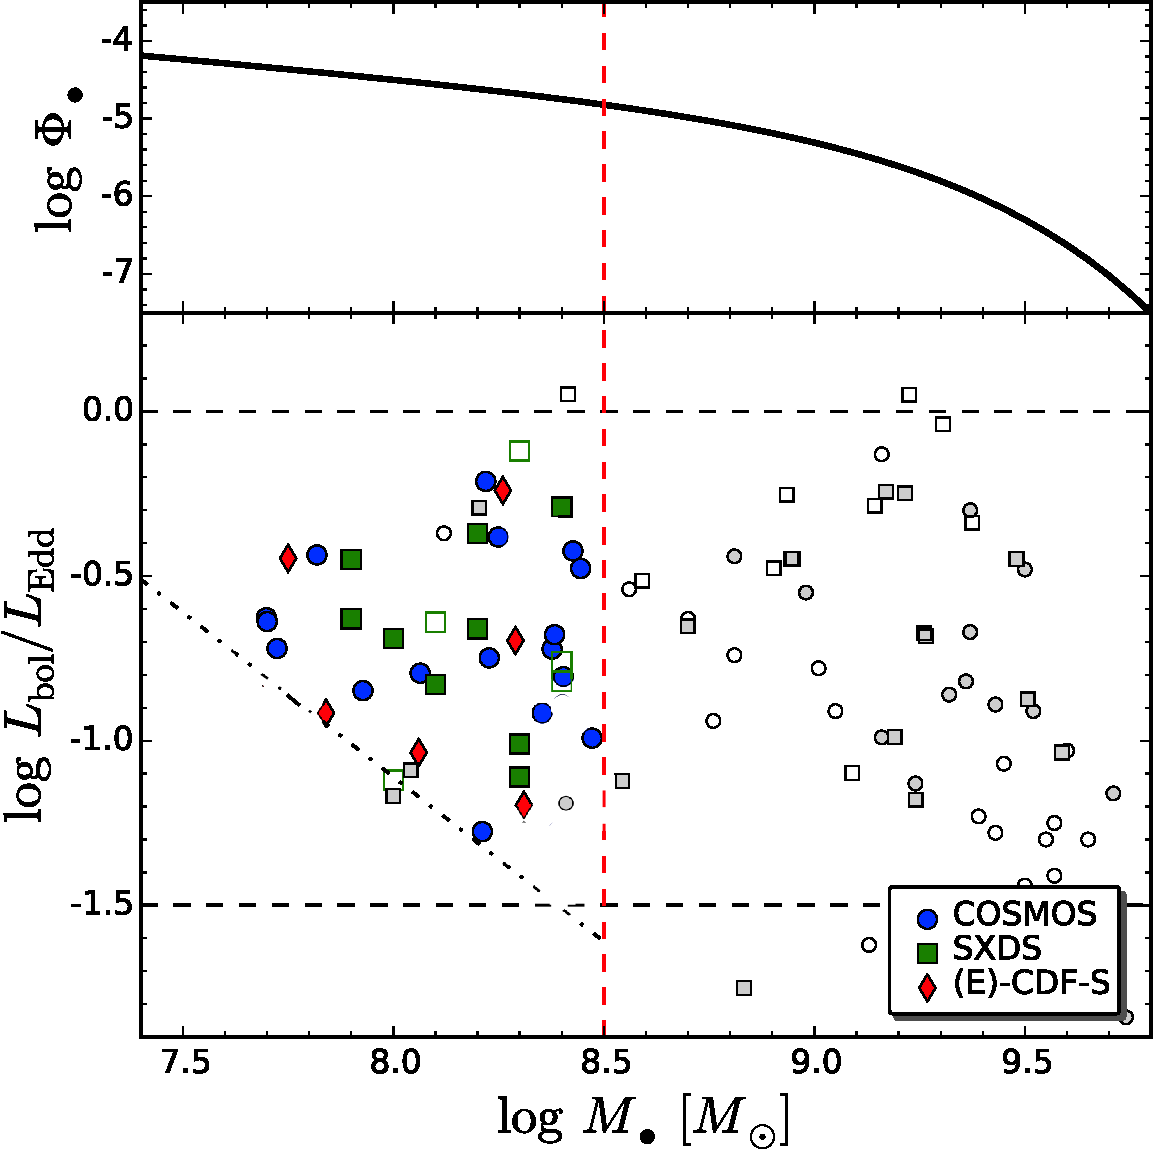
\includegraphics[width=0.8\linewidth]{hst_sample_bhmf.pdf}
%\caption{
%The selection function of our observation data. Eddington ratios (LBol/LEdd) and BH masses (bottom panel) of our sample (in color) that fall well-below the knee of the BH mass function at z = 1.5 (top panel; Schulze et al. 2015). Dashed lines (vertical and horizontal) denote our selection window with the slanted line only shown to approximately illustrate the effect of a luminosity limit, inherent in the parent catalogs. For reference, we indicate the high-z luminous SDSS QSO samples (grey squares - Peng et al. 2006; grey circles - Decarli et al. 2010) with all falling above our chosen upper mass limit.
%}
%\label{fig:support}
%\end{center}
%\end{figure}

\end{document}
